\section{Auswertung}
\label{sec:Auswertung}

\subsection{Freie Weglänge}

Mithilfe der Gleichungen \ref{eqn:Temperatur} und \ref{eqn:Sättigungsdampfdruck} wird die mittlere freie Weglänge
berechnet, die die Teilchen besitzen.

\begin{table}[H]
    \centering
    \label{tab:weg}
    \caption{Das Verhältnis der mittleren freien Weglänge zu dem Abstand zwischen der Kathode und Beschleunigungselektrode
            $a$ bei den entsprechenden Temparaturen.}
    \begin{tblr}{
        colspec={S   S   S    S  S},
        row{1}={guard,mode=math},
        vline{3}={2}{-}{text=\clap{e}}
    }
    \toprule
    T \text{/}\unit{\kelvin}    &   w/a \text{/}\unit{\meter} &  \\
    \midrule
    297.55  &   5.73    &   0    \\
    423.15  &   6.01    &   -3    \\
    433.15  &   4.13    &   -3    \\
    449.15  &   2.35    &   -3    \\
    468.15  &   1.26    &   -3    \\
    \bottomrule
    \end{tblr}
\end{table}
%Der erste Wert ist als inakkurat zu verwerfen, da w/a<10^(-3) sein muss, damit die berechnung stimmt. außerdem musst du
%einen Faktor in der Theorie korrigieren. Du warst eine Größenordnung zu groß für die Weglänge

\subsection{Kontaktpotential}
\begin{figure}[H]
    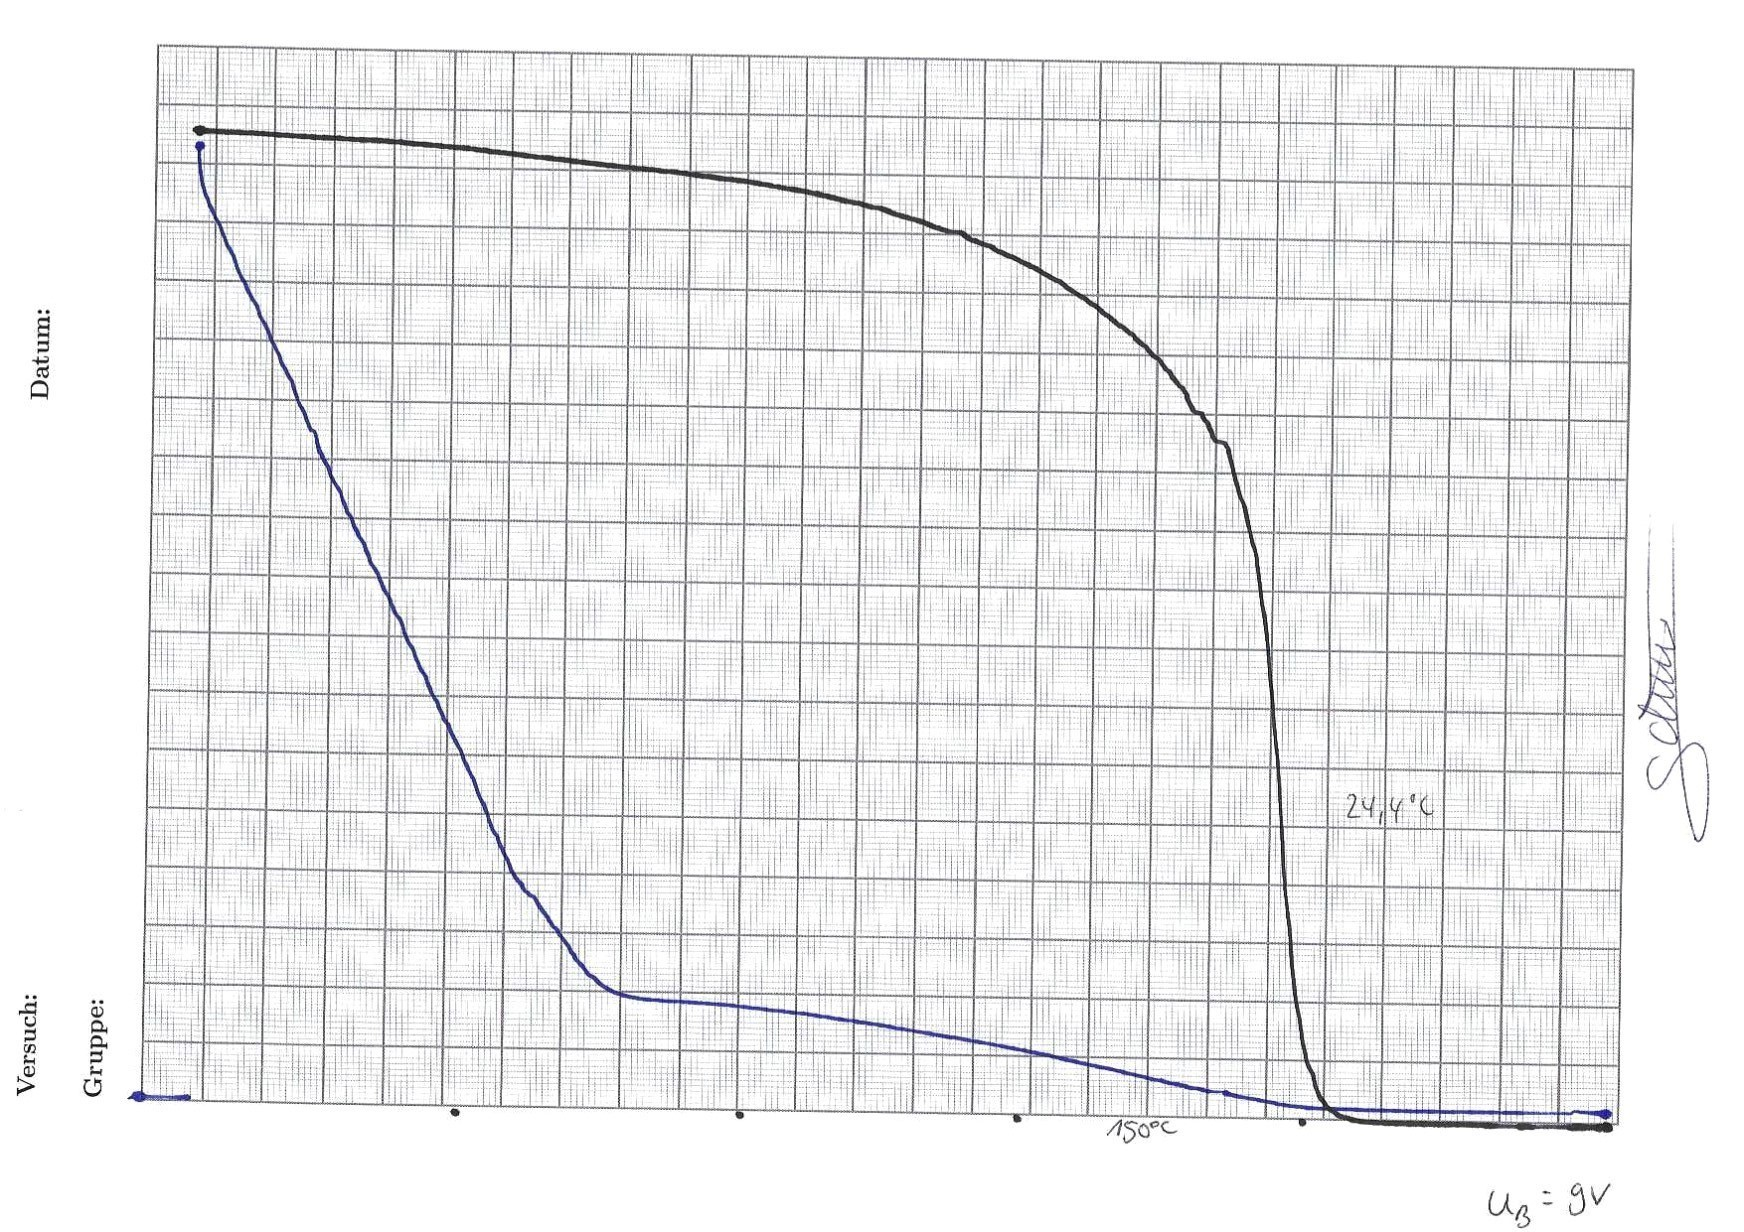
\includegraphics[width=\textwidth]{Bilder/1.jpg}
    \caption{Gemessene Stromstärke gegen die Abbremsspannung bei unterschiedlichen Temparaturen und konstanter Beschleunigungsspannung
    $U_B=\qty{11}{\volt}$.}
    \label{fig:1}
\end{figure}

Die maximale Abfall der gemessenen Stromstärke liegt nach Abbildung \ref{fig:1} bei ungefähr $U_G=\qty{1.80(0.9)}{\volt}$.
Dabei wird hier nur der Messbereich zwischen 6 und 8 Volt betrachtet, da sich dort der relevante Abfall befindet. In diesem
Intervall entspricht 1 Volt etwa $\qty{2.5}{\centi\meter}$. Nach Gleichung \ref{eqn:Kontaktpotential} beträgt das 
Kontaktpotential dann $K=\qty{1.2(0.09)}{\electronvolt}$.

%das Kontaktpotential ist die Verschiebung von der angelegten Beschleunigungsspannungdem zum maximalen Abfall der Stromstärke

\begin{figure}[H]
    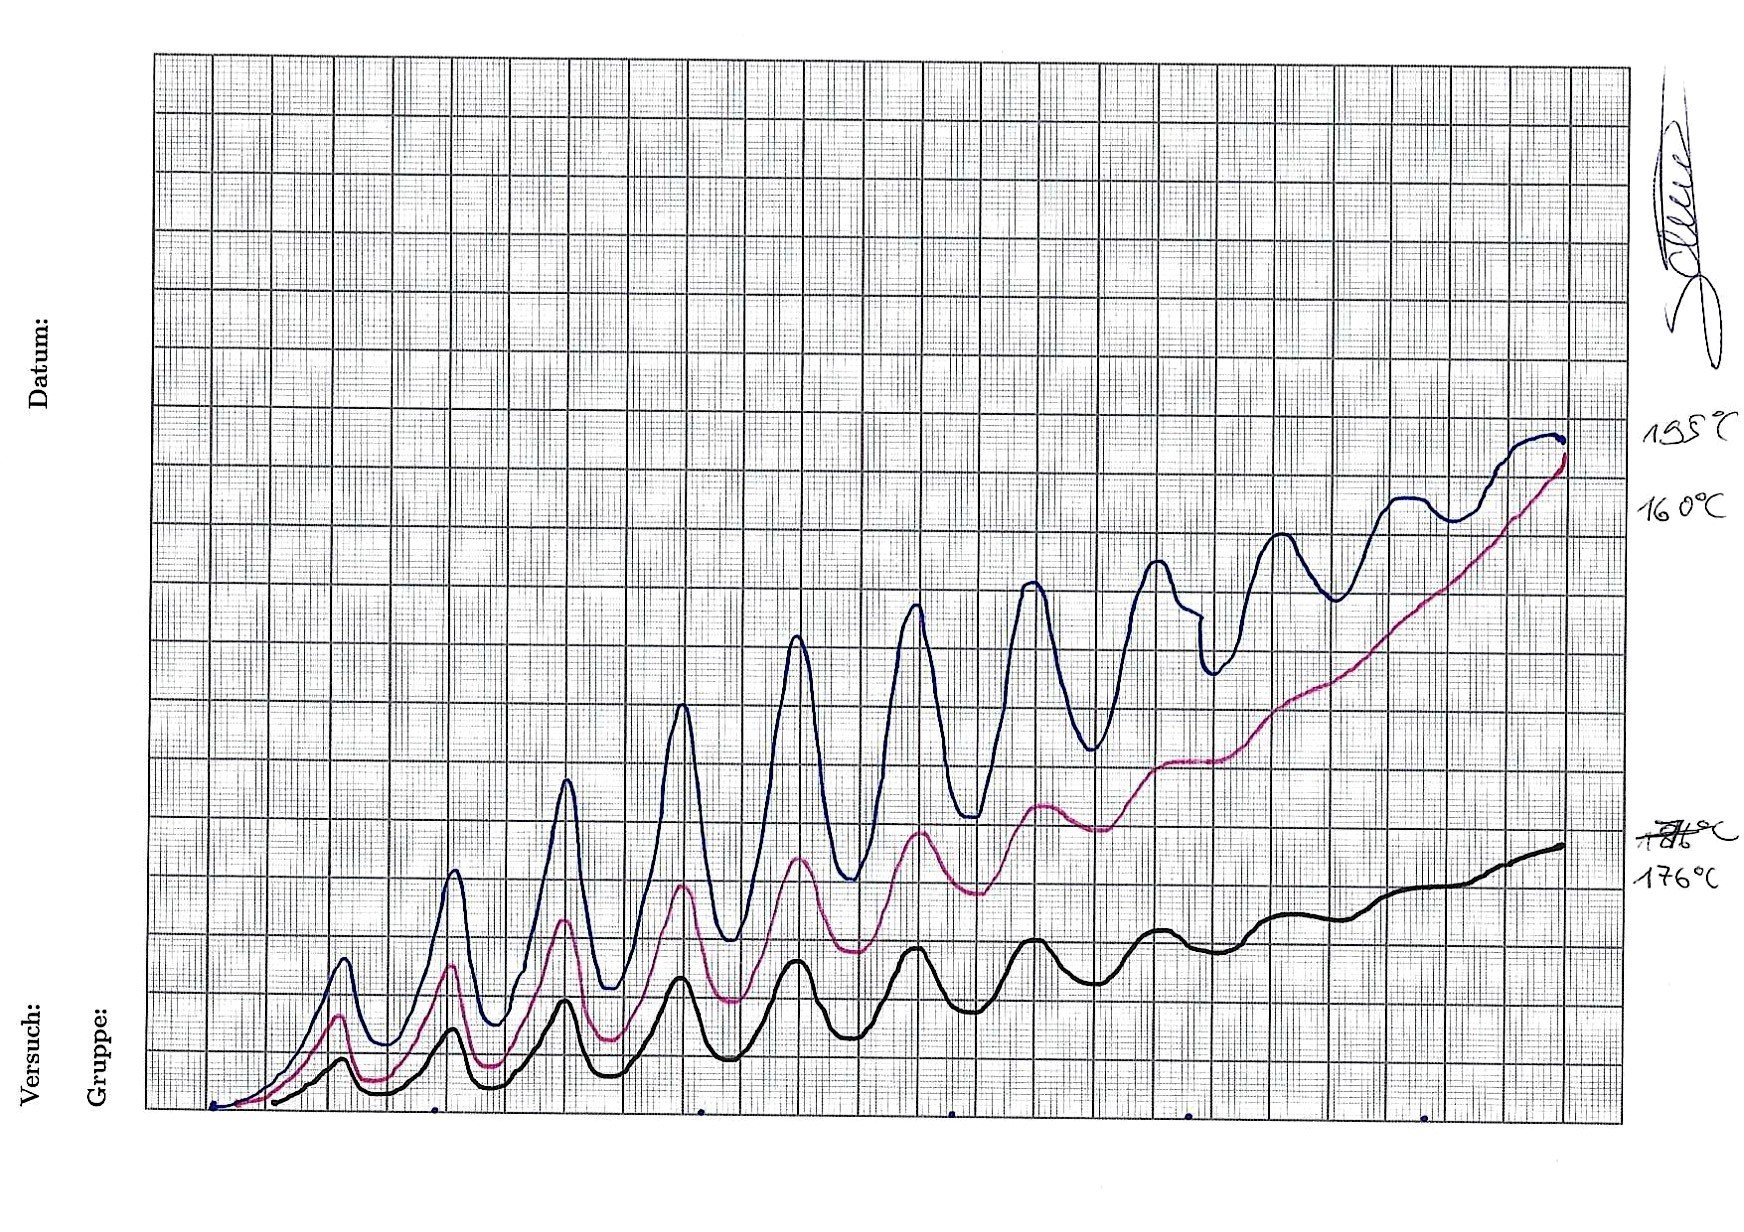
\includegraphics[width=\textwidth]{Bilder/2.jpg}
    \caption{Gemessene Stromstärke gegen die Beschleunigungsspannung bei unterschiedlichen Temparaturen und konstanter Bremsspannung
    $U_A=\qty{1}{\volt}$.}
    \label{fig:2}
\end{figure}

Anhand der Abbildung \ref{fig:2} ist feststellbar, dass der Abstand zwischen den Maxima $d=\qty{2.1(0.1)}{\centi\meter}$, 
wobei $\qty{1}{\volt}$ gemittelt $\qty{0.424(0.004)}{\centi\meter}$ entspricht. Somit beträgt die Spannungsdifferenz 
$\delta U=\qty{0.89(0.04)}{\volt}$. Diese Bestimmung ist für alle drei Graphen, da deren lokale Maxima überlappen.\\

Die zu der Energie entsprechenden Wellenlänge beträgt $\lambda=\qty{1.39(0.07)e-6}{\meter}$.

%ich bin mir hier nicht sicher, ob ich die richtige Spannung verwendet habe. Ich habe die Differenz verwendet, die Wellenlänge kommt mir aber zu groß vor.